% Copyright (c) 2014,2016 Casper Ti. Vecto
\chapter{系統概要設計} 


	本論文提出比特幣的交易監督系統(Bitcoin Transaction Monitoring System,BTMS)\supercite{Blockchain-basedpaymentcollectionsupervisionsystemusingpervasiveBitcoindigitalwallet},以下簡稱BTMS,BTMS以加密貨幣比特幣實作,BTMS包含三個子系統,商家和商品信息管理子系統(Store and Merchandise Information Management Sub-System,SMIMSS)、商家移動裝置收款及交易子系統(Store Mobile payment Collection and Transaction Sub-System,SMCTSS)、客戶端行動支付和交易子系統(Client Mobile Payment and Transaction Sub-System,CMPTSS),圖\ref{model0}為主系統與子系統的功能模塊圖。

	\begin{figure}[!htbp]
		\centering
		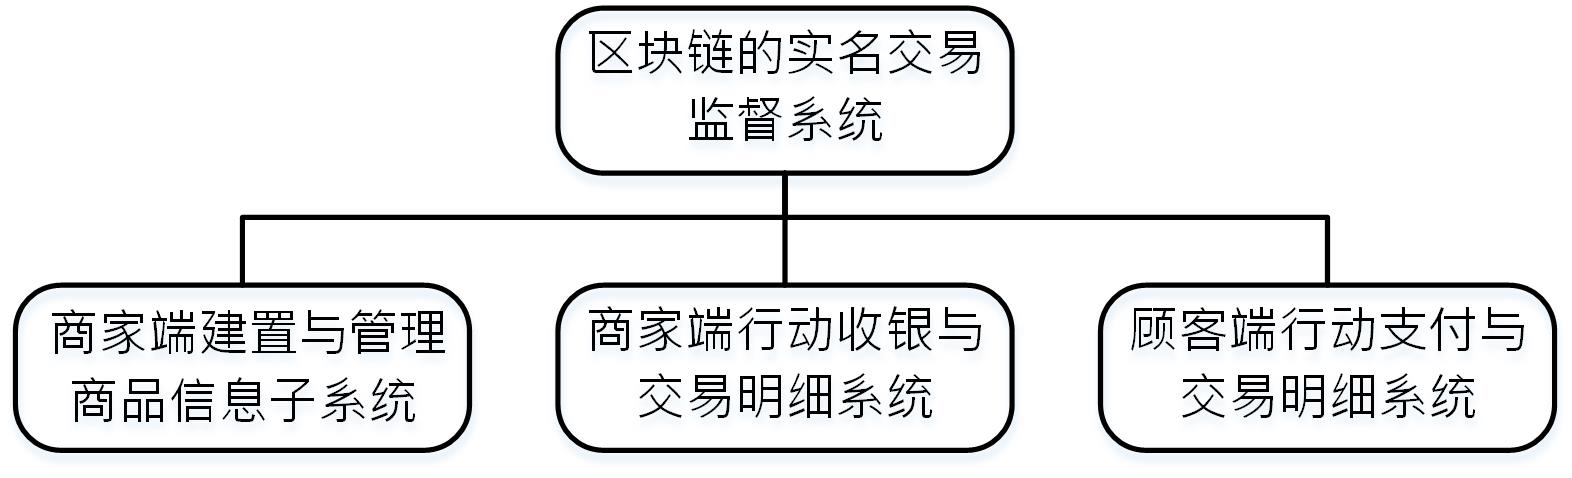
\includegraphics[width = 0.8\textwidth]{model0.jpg}
		\caption{BTMS系統功能模塊圖}\label{model0}
	\end{figure}

	本論文設計讓商家能夠結合商品與RFID標籤,以達到快速建構與管理商品數據庫之系統,並且讓商家及顧客可以運用手機NFC功能來實際運作比特幣的行動支付流程。商家只需要掃描商品上的RFID標籤,即可快速建立交易清單,再利用NFC功能與顧客之行動裝置進行信息交換,輕鬆地將商家的收款地址以及交易資料傳送給顧客,收到資料後便能快速地以顧客之比特幣行動電子錢包付款,並將交易細項儲存下來,以便未來商家與顧客能夠快速查詢比特幣行動支付的交易記錄。
	本系統主要是以完成區塊鏈之加密貨幣的收款監督系統為主要目標,本論文進而將積極利用自由軟體的利基:使用成本低、進入門檻低、開放原始碼、社群能力強、共通性及移植性強、資通安全性高等優勢來開發本論文收款監督系統的應用服務平台。本系統範圍包含建置下各項子系統如下:
		\begin{enumerate}
		\item 商家和商品信息管理子系統(Store and Merchandise Information Management Sub-System,SMIMSS):本系統可以讓商家在進貨時,快速地將RFID標籤之識別碼與進貨商品資訊集成在一起,並且透過本系統新增、修改或刪除資料庫內部的資訊,包括產品名稱、詳細資訊,存貨數量等資訊,商家與顧客便可依照該資料庫取得當前商品資訊與狀態。不僅讓商家的存貨資訊更加清楚明瞭,也可以提供顧客更多的即時服務,圖\ref{model1}所示。

			\begin{figure}[!htbp]
			\centering
			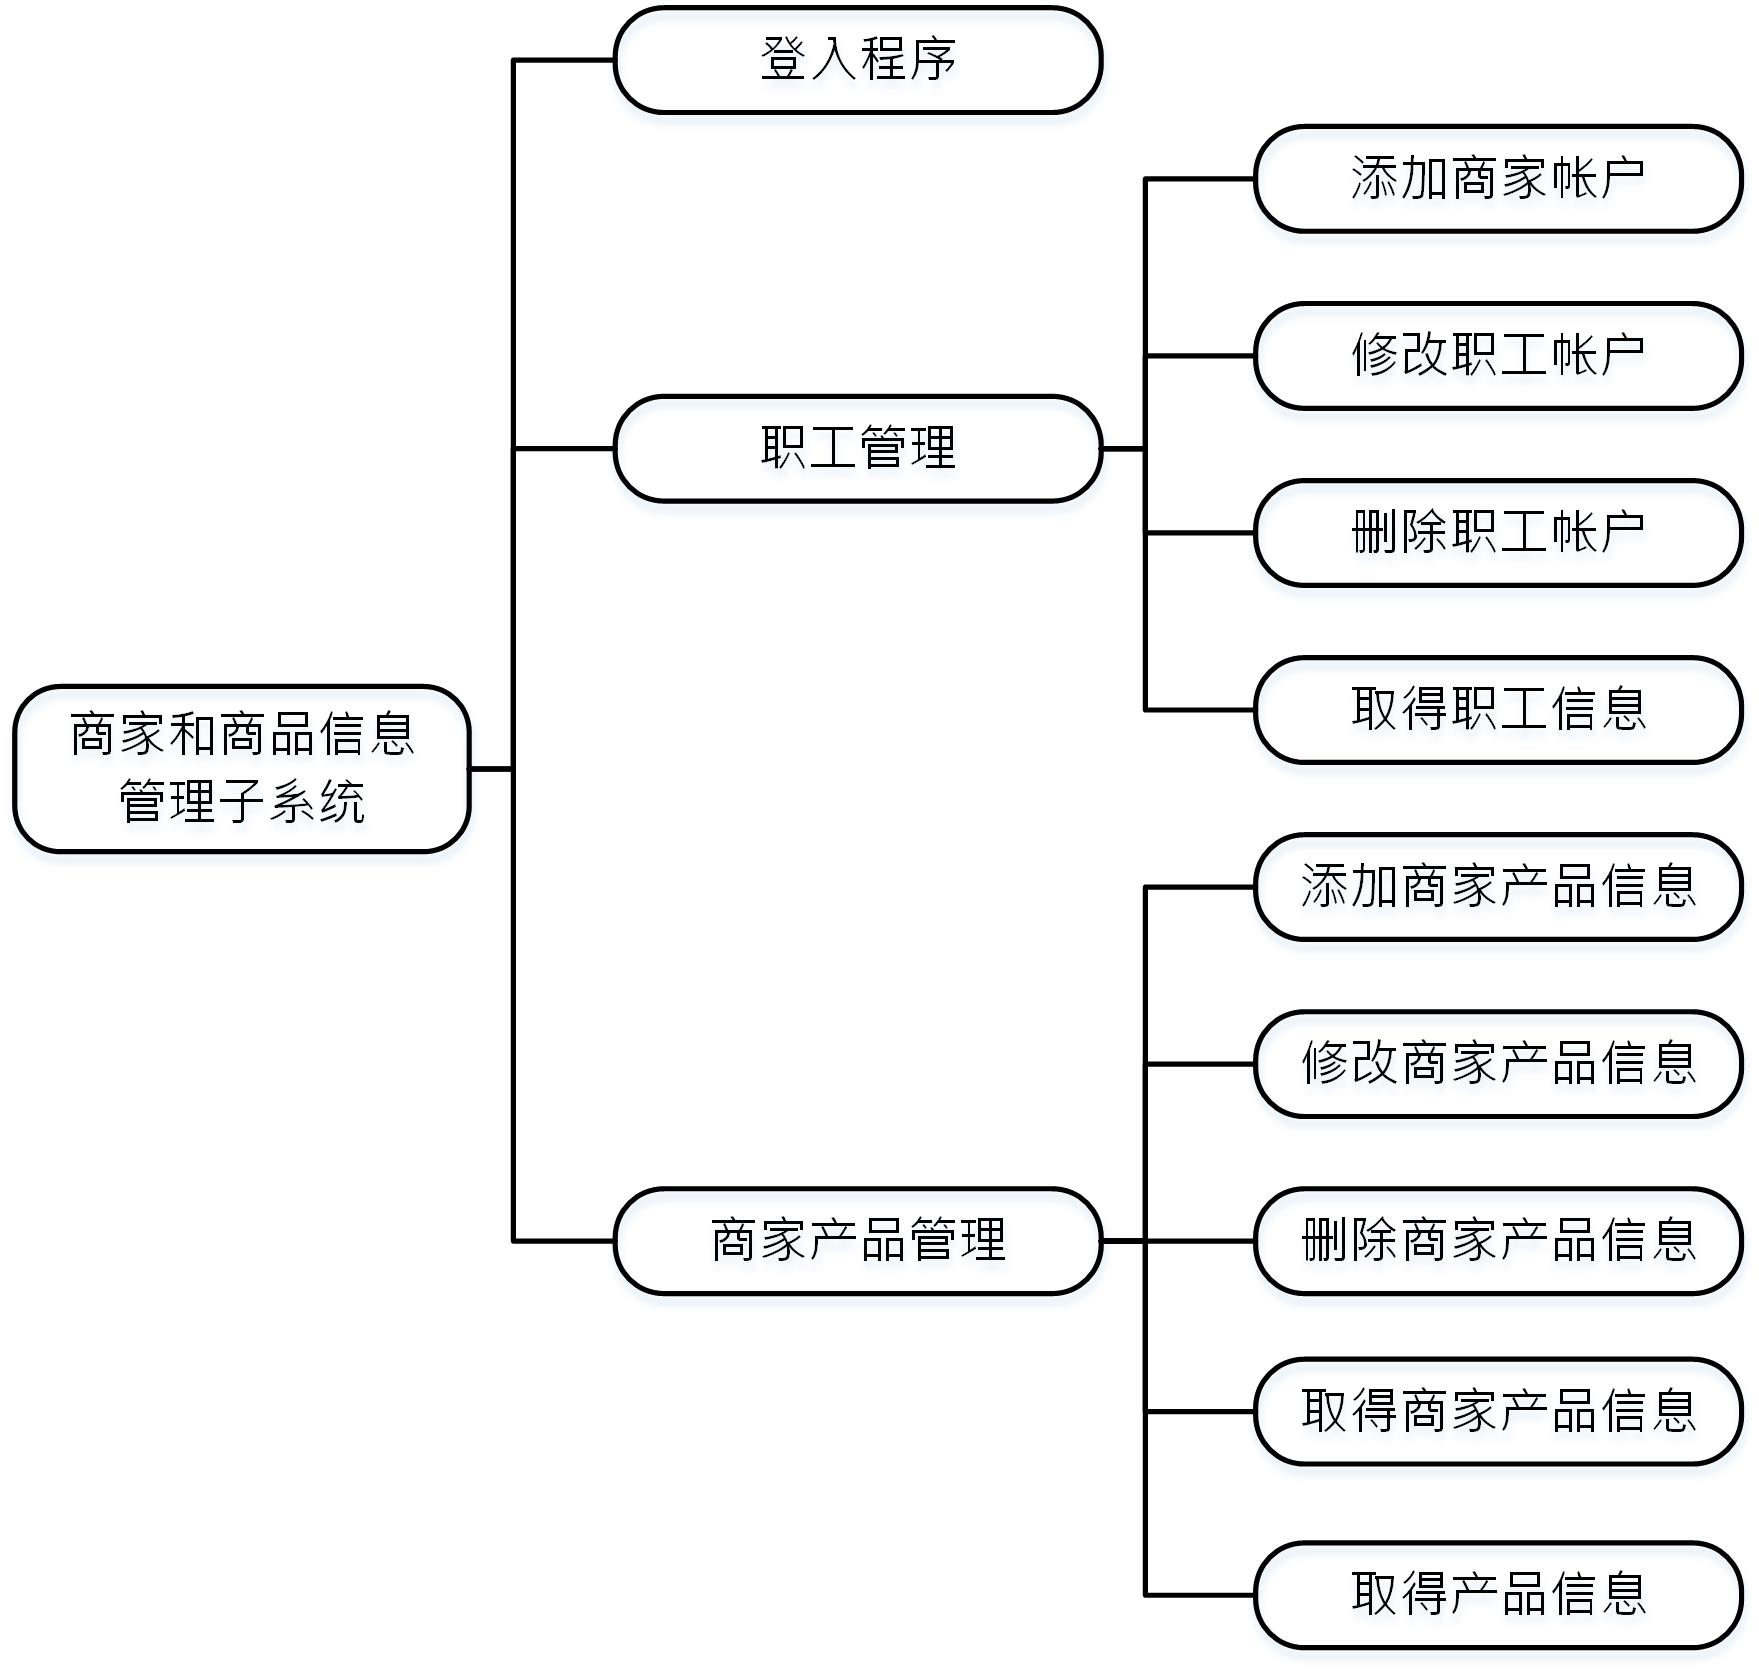
\includegraphics[width = 0.7\textwidth]{model1.jpg}
			\caption{商家和商品信息管理子系統功能模塊圖}\label{model1}
			\end{figure}



		\item 商家移動裝置收款及交易子系統(Store Mobile payment Collection and Transaction Sub-System,SMCTSS):本系統使商家在結帳時,能夠以手機NFC功能掃描商品上的RFID 標籤,即可簡單地建立交易清單,並透過NFC與顧客手機碰觸,將交易清單以及商家之比特幣收款地址等等重要交易資訊一併傳遞給顧客,可以減短結帳的速度,使結帳效率大幅提升,圖\ref{model3}所示。
		 
			\begin{figure}[!htbp]
			\centering
			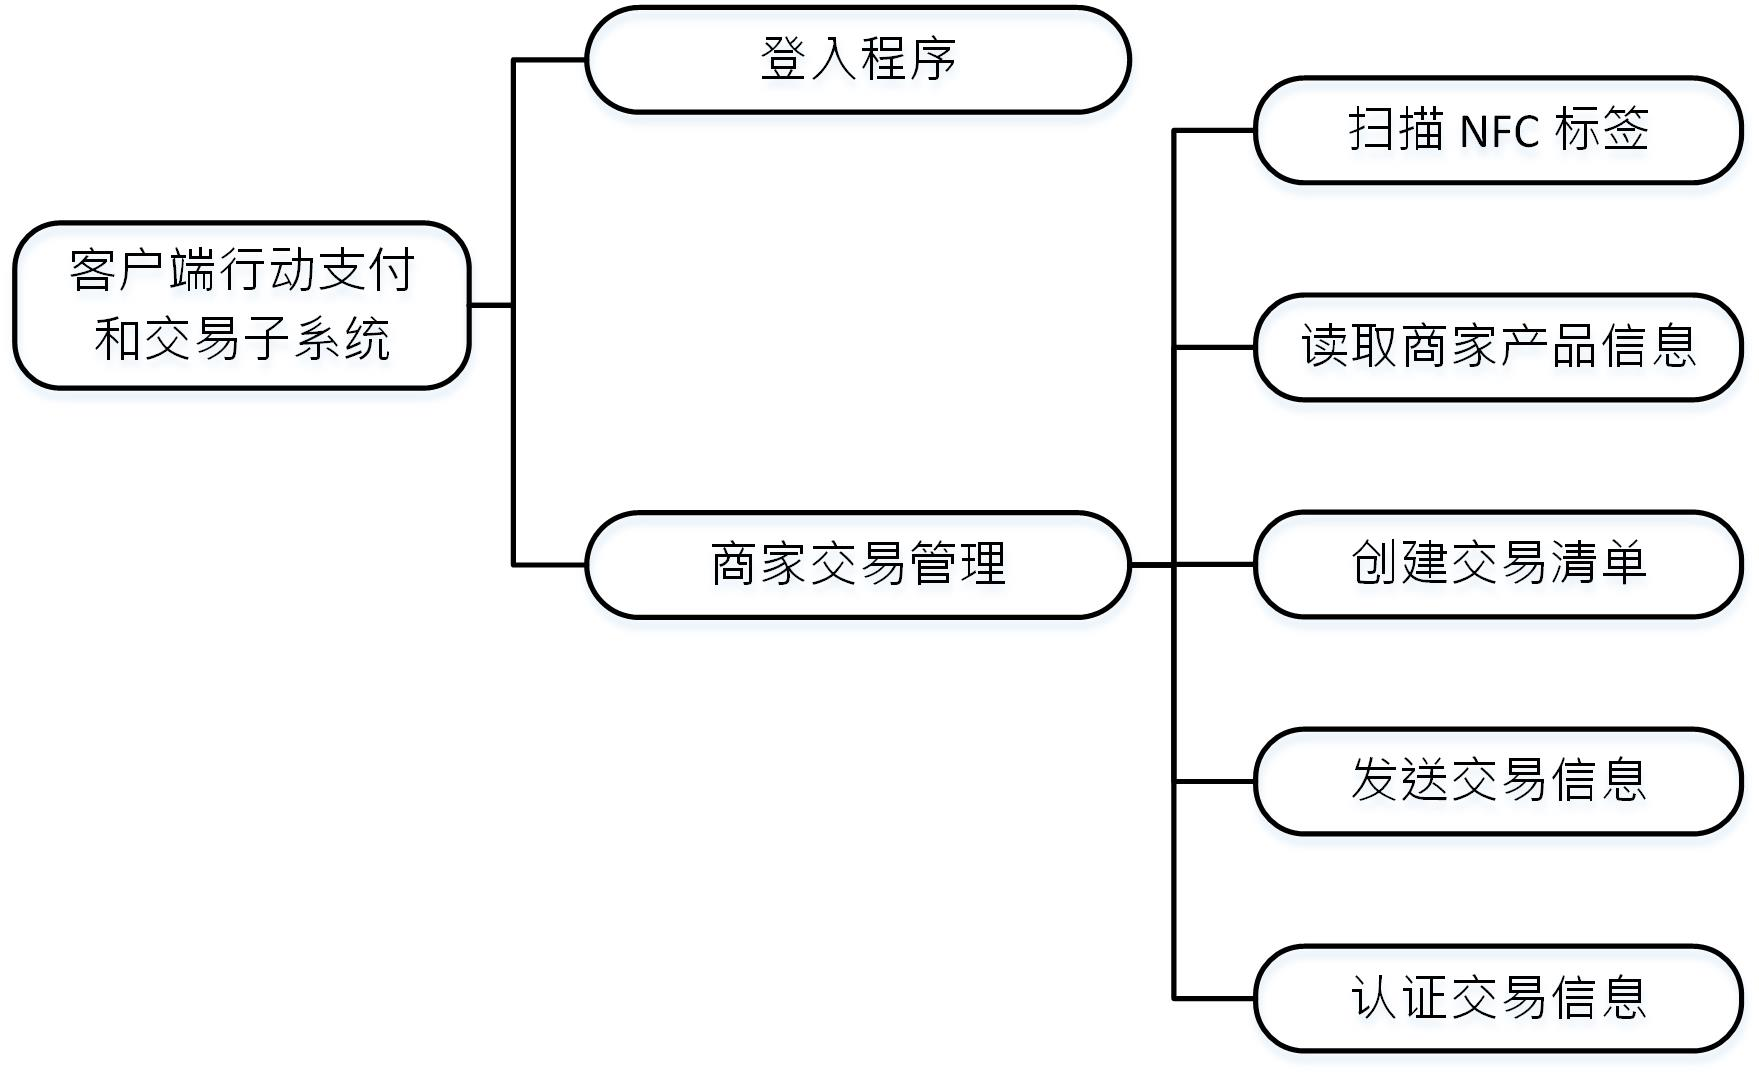
\includegraphics[width = 0.7\textwidth]{model3.jpg}
			\caption{商家移動裝置收款及交易子系統功能模塊圖}\label{model3}
			\end{figure}


		\item 客戶端行動支付和交易子系統(Client Mobile Payment and Transaction Sub-System,CMPTSS):顧客在結帳時,不必再麻煩的拿出信用卡或是零錢包,只需要拿出手機讓職工以NFC將交易清單與比特幣地址轉送給自己,即可自動連結至比特幣電子錢包的應用程式當中,並且自動填妥相關資料,如:交易金額、收款地址等等與此同時也能將交易紀錄儲存於客戶端,以便日後顧客快速取得過往的交易紀錄,除此之外亦可讓廣大的民眾體驗加密貨幣與行動支付帶來的便利生活,圖\ref{model2}所示。
			\begin{figure}[!htbp]
			\centering
			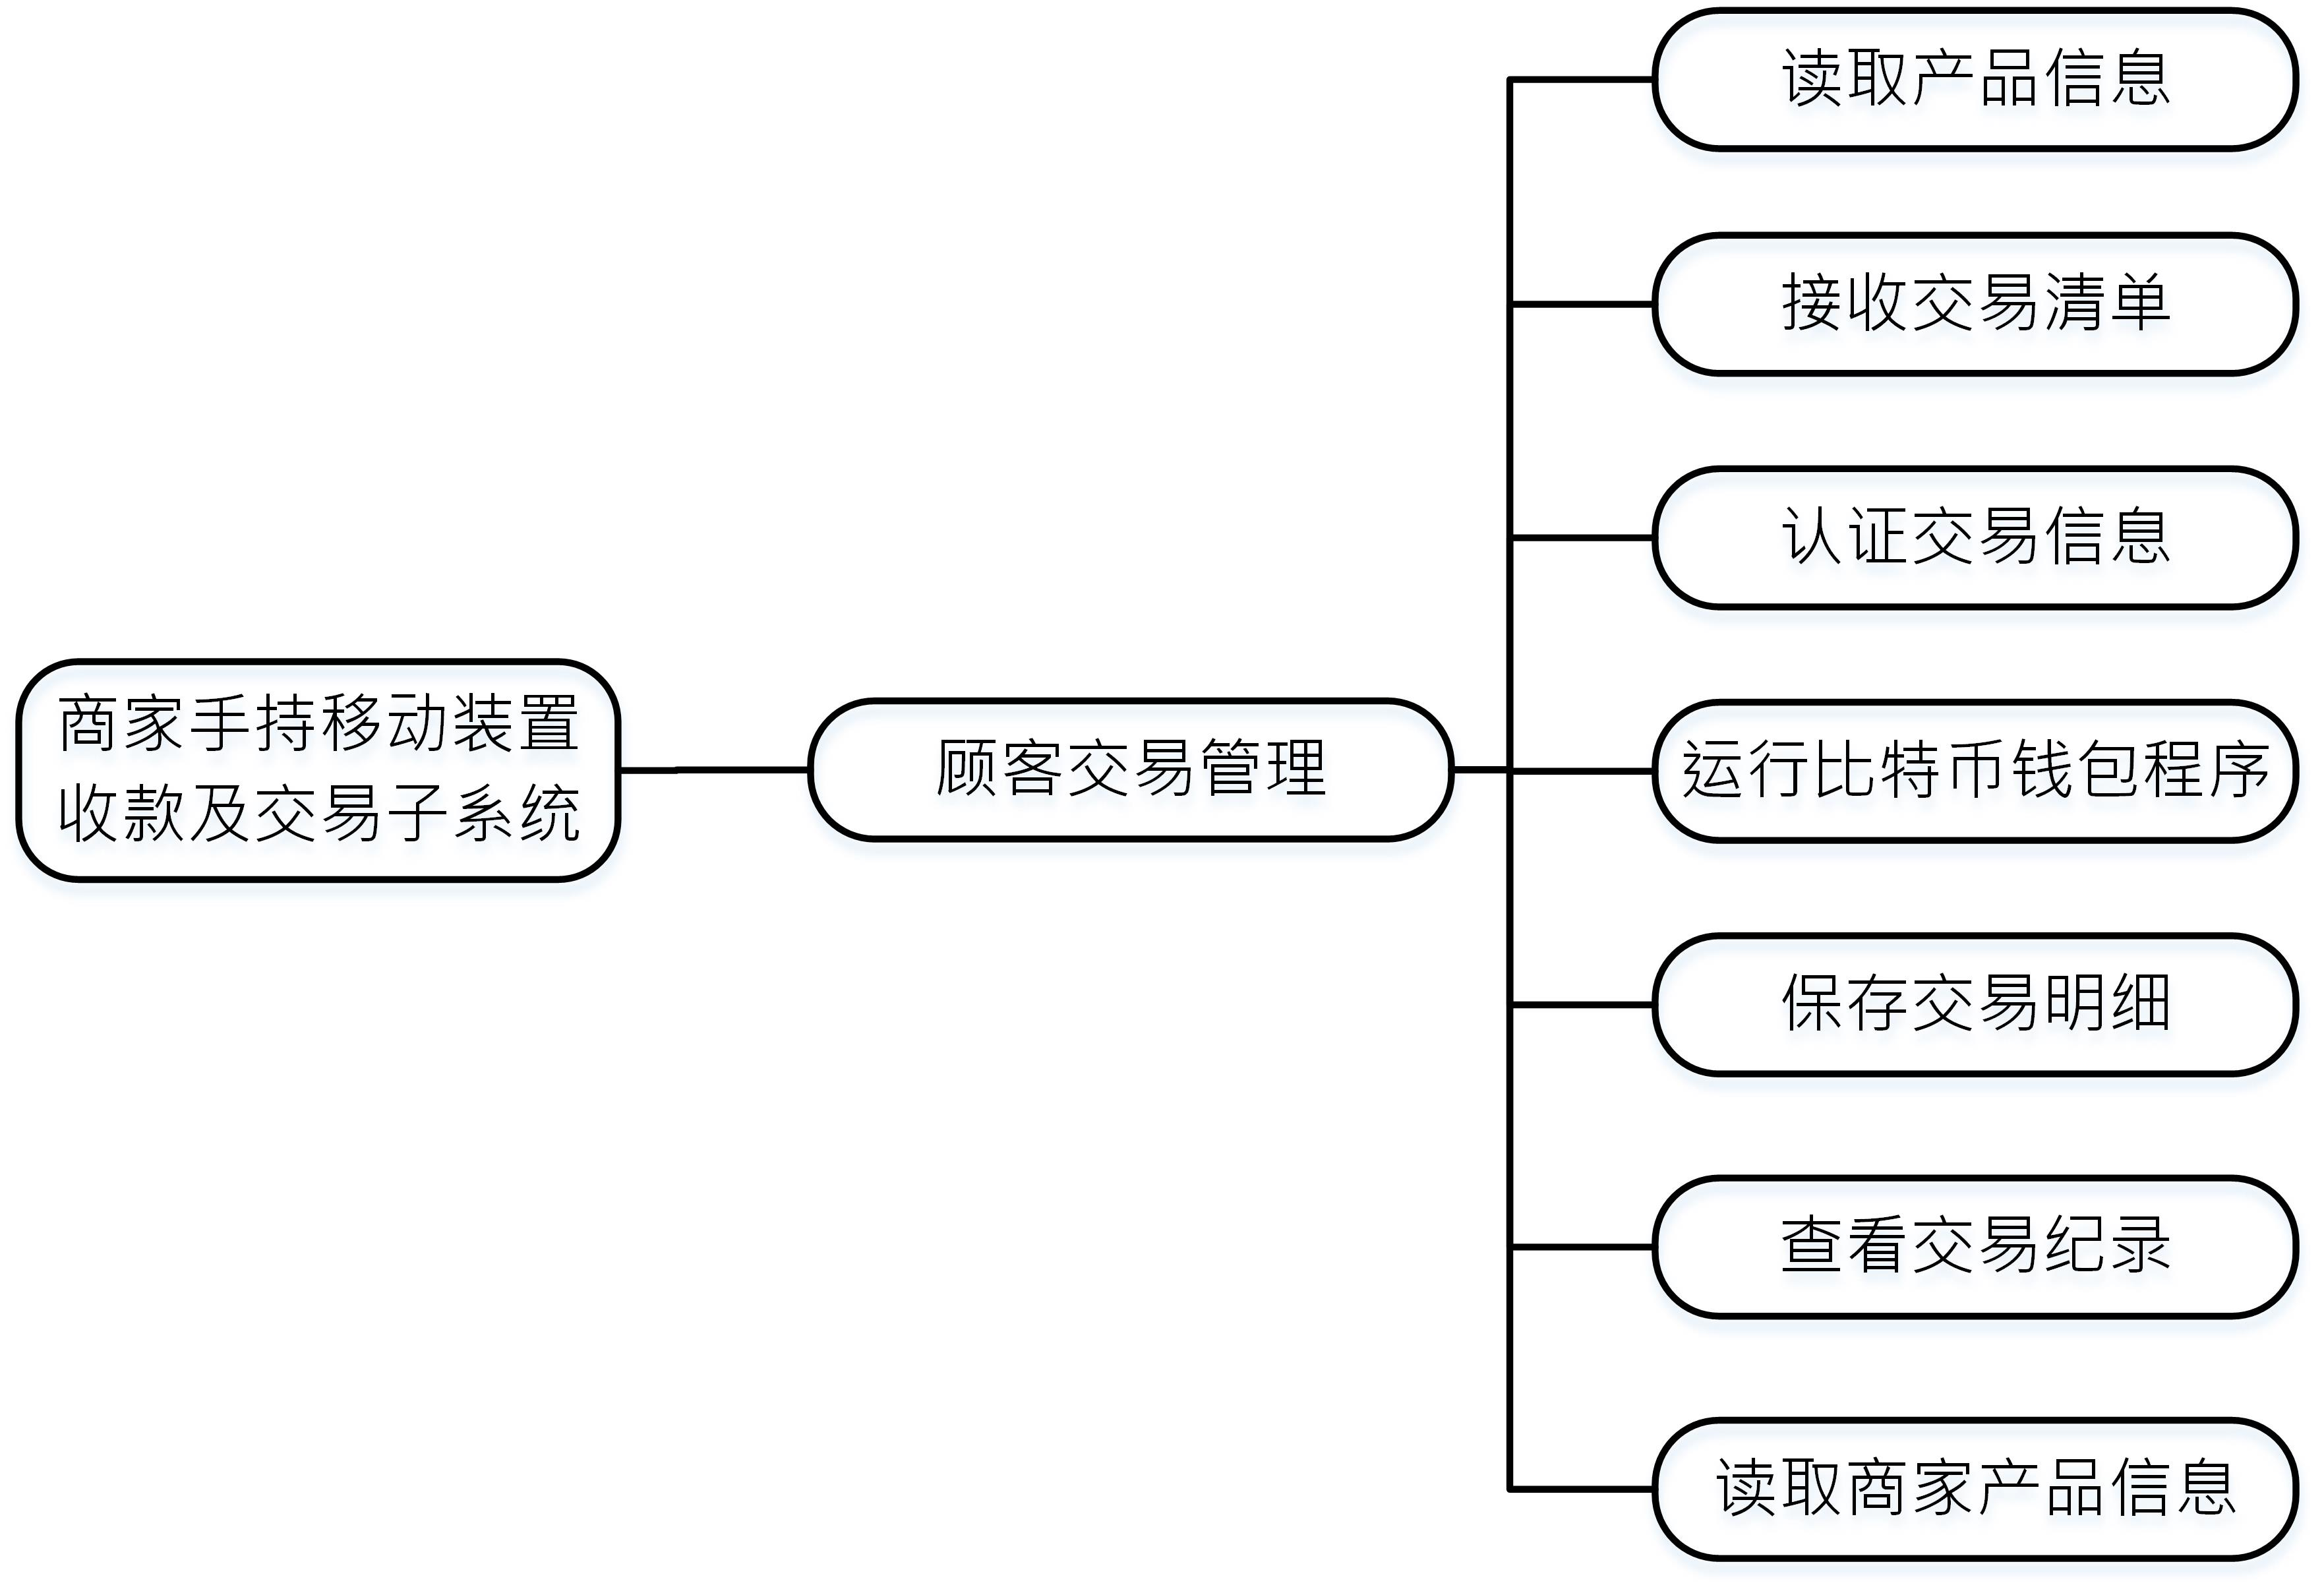
\includegraphics[width = 0.7\textwidth]{model2.jpg}
			\caption{客戶端行動支付和交易子系統功能模塊圖}\label{model2}
			\end{figure}
		
	\end{enumerate}
	

\section{BTMS架構與運作流程}

	圖\ref{fig3}為BTMS和商家註冊流程架構圖,商家需要在以下4個步驟中對用戶註冊與登入:

	\begin{figure}[!htbp]
		\centering
		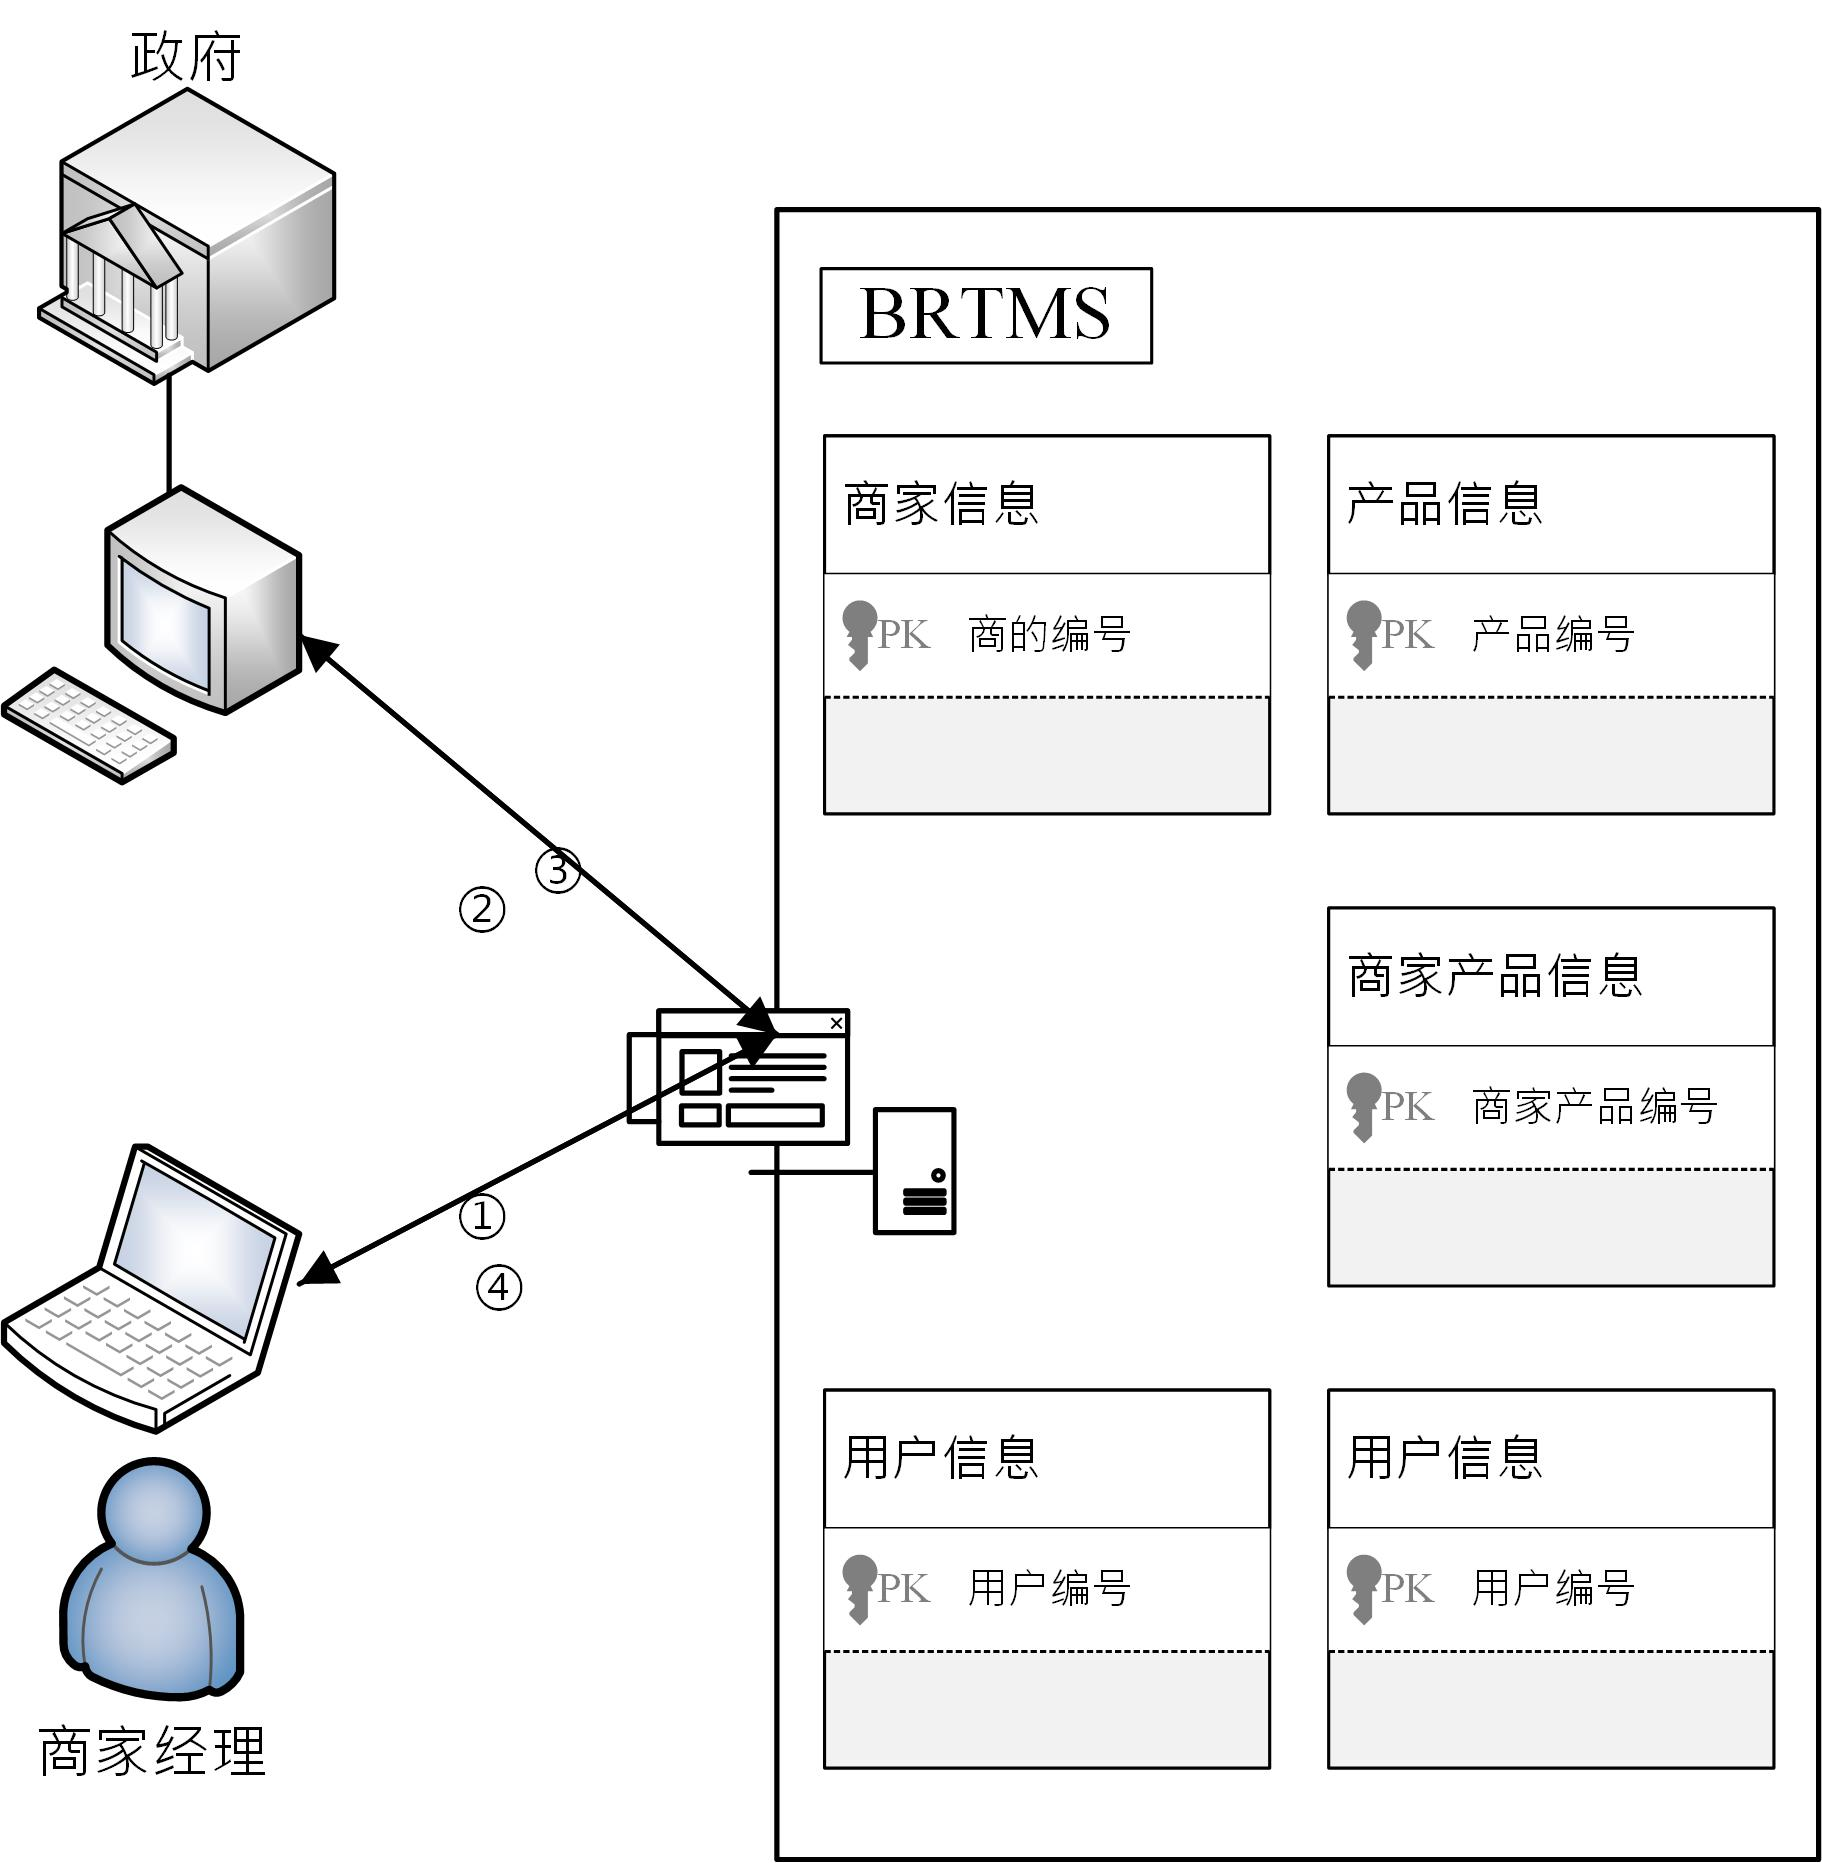
\includegraphics[width = 0.6\textwidth]{fig3.jpg}
		\caption{BTMS和商家註冊流程架構圖}\label{fig3}
	\end{figure}

	\begin{enumerate}
		\item 商家必須在BTMS註冊一個用戶,並附有政府法規的商業證明。
		\item 比特幣的交易監督系統將自動向相應的政府金融監管機構提交商業申請,以審查該商家的加密貨幣交易業務。
		\item 如果政府批准商家的加密貨幣業務申請,服務器將激活商家在該收集監控系統中創建商家用戶。
		\item 商家可以自由地登錄帳戶並添加商家想要出售的產品信息,亦可透過職工管理添加修改刪除職工信息。
	\end{enumerate}

	具體的加密貨幣商家收銀金流監控系統運行過程如圖\ref{fig4}所示,以圖\ref{fig3}所設計出的系統架構進行擴增,首先需要與區塊鏈檢視器 (Blockchain Explorer)\supercite{Blockchainexplorer:Ananalyticalprocessandinvestigationenvironmentforbitcoin}對接,而之所以該監控系統需要與區塊鏈檢視器對接是為了能夠最直接的比對交易被記錄的成交狀況,能夠達到即時性以及正確性,倘若擔憂單方面的依賴相信區塊鏈檢視器的成果,亦可以使用多家區塊鏈檢視器進行交叉參考,以避免因為一家公司的錯誤所帶來的影響。區塊鏈檢視器的目的是為了能夠快速地準確地比對該筆交易的成交,做為整筆交易提出到結算的環節之一。

	\begin{figure}[!htbp]
		\centering
		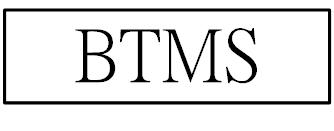
\includegraphics[width = 0.8\textwidth]{fig4.jpg}
		\caption{BTMS的整體架構與功能示意圖}\label{fig4}
	\end{figure}

	圖\ref{fig4}比特幣的交易監督系統創建步驟描述如下:

		\begin{enumerate}
			\item 商家職工將登錄到圖\ref{fig3}中的第一個步驟,所示的先前步驟創建的用戶,使用手持式平板電腦或智能手機訪問SMCTSS中的服務。如前所述,在能夠登錄到系統之前,商家用戶必須由政府機構審計。
			\item 在成功登錄SMCTSS用於商家加密貨幣金流監控系統時,移動設備將加載通過SMIMSS註冊的商家產品信息,然後創建產品目錄。商家的職工可以根據顧客的需求選擇所需的產品和數量。

			\item 職工使用設備完成顧客選定商品的產品信息後,移動設備上的NFC技術可用於將產品信息從附近職工的移動設備傳遞給顧客的移動設備,而無需物理交互。然後,顧客可以很容易地將自己的消費信息記錄成為發票等參考。在接收從商家職工設備向顧客設備購買產品信息之後,顧客設備將向商家的移動設備發送其自己的比特幣支付地址的信息。
			\item 商家的手持設備收到顧客確認購買所選產品的相應信息後,會將交易信息的副本發送給SMIMSS監控系統。顧客信息包括交易序列號、商家ID號碼、商品號碼、購買的商品的數量以及加密貨幣的收款人地址以及顧客的支付地址。
			\item 收到顧客交易信息後,即完成此次的加密貨幣支付。同時,此次交易的加密貨幣將透過客戶端CMPTSS發布到比特幣網絡中進行驗證和記錄。
			\item 區塊鏈檢視器將開始分析在比特幣網絡中緩存池的所有交易以及區塊鏈中記錄的交易。
			\item 擬議的交易監控系統BTMS將向區塊鏈檢視器提出請求。這個請求數據不僅包括存儲在BTMS中的交易副本之加密貨幣收款人地址,如圖\ref{fig4}的第四步驟,還包括顧客預期付款的加密貨幣支付地址。區塊鏈檢視器使用請求數據來檢查交易是否存儲在區塊鏈中,或者交易還在等待確認。如果交易已被確認並存儲在區塊鏈中,則交易數據庫中"交易確認"字段的值將更改為"1",否則其默認值為"0"。
			\item 當"交易確認"字段中的值為"1"時,"交易已完成"消息可發送至商家平板電腦上運行的商家和商品信息管理子系統(SMIMSS)。
			\item 政府財政監督部門可以審查擬議BTMS中的所有交易信息,以作為稅收審計參考。
		\end{enumerate}

\section{實時BTMS架構與運作流程}

		在BTMS的機制前提下,提出比特幣多重簽章算法實踐於政府端,將該方法稱為Government Green Address,將優化後的系統稱為比特幣的實時交易監督系統(Bitcoin Real-time Transaction Monitoring System,BRTMS),以下則將該實時系統簡稱為BRTMS,BRTMS與過去Green Address 比特幣錢包地址不同的在於Green Address生成需要生成兩把私鑰分別為用戶私鑰以及Green Address 機構的私鑰,並將兩把私鑰加以合併形成Green Address錢包地址。在用戶發起基於Green Address機制的比特幣交易時,用戶生成交易並使用數字簽名,再將該筆交易發送至Green Address機構進行下一個步驟的數字簽名,在這過程中完成Green Address機制交易必需依賴Green Address機構,且該機構位於海外,在封包傳輸上會有一定程度的延遲。為了提升國內用戶可以更快速地透過多重簽章技術提升交易速度,BRTMS將取代原有的Green Address機構,使得國內的用戶擁有更快的網路傳輸速度,更快的完成多重簽章算法簽名。\supercite{tanet}。 

本節將詳述本系統之商家註冊、Government Green Address錢包創建與驗證交易的運作流程與相關數據庫架構,如圖\ref{gabpcss}所示。

	\begin{figure}[!htbp]
		\centering
		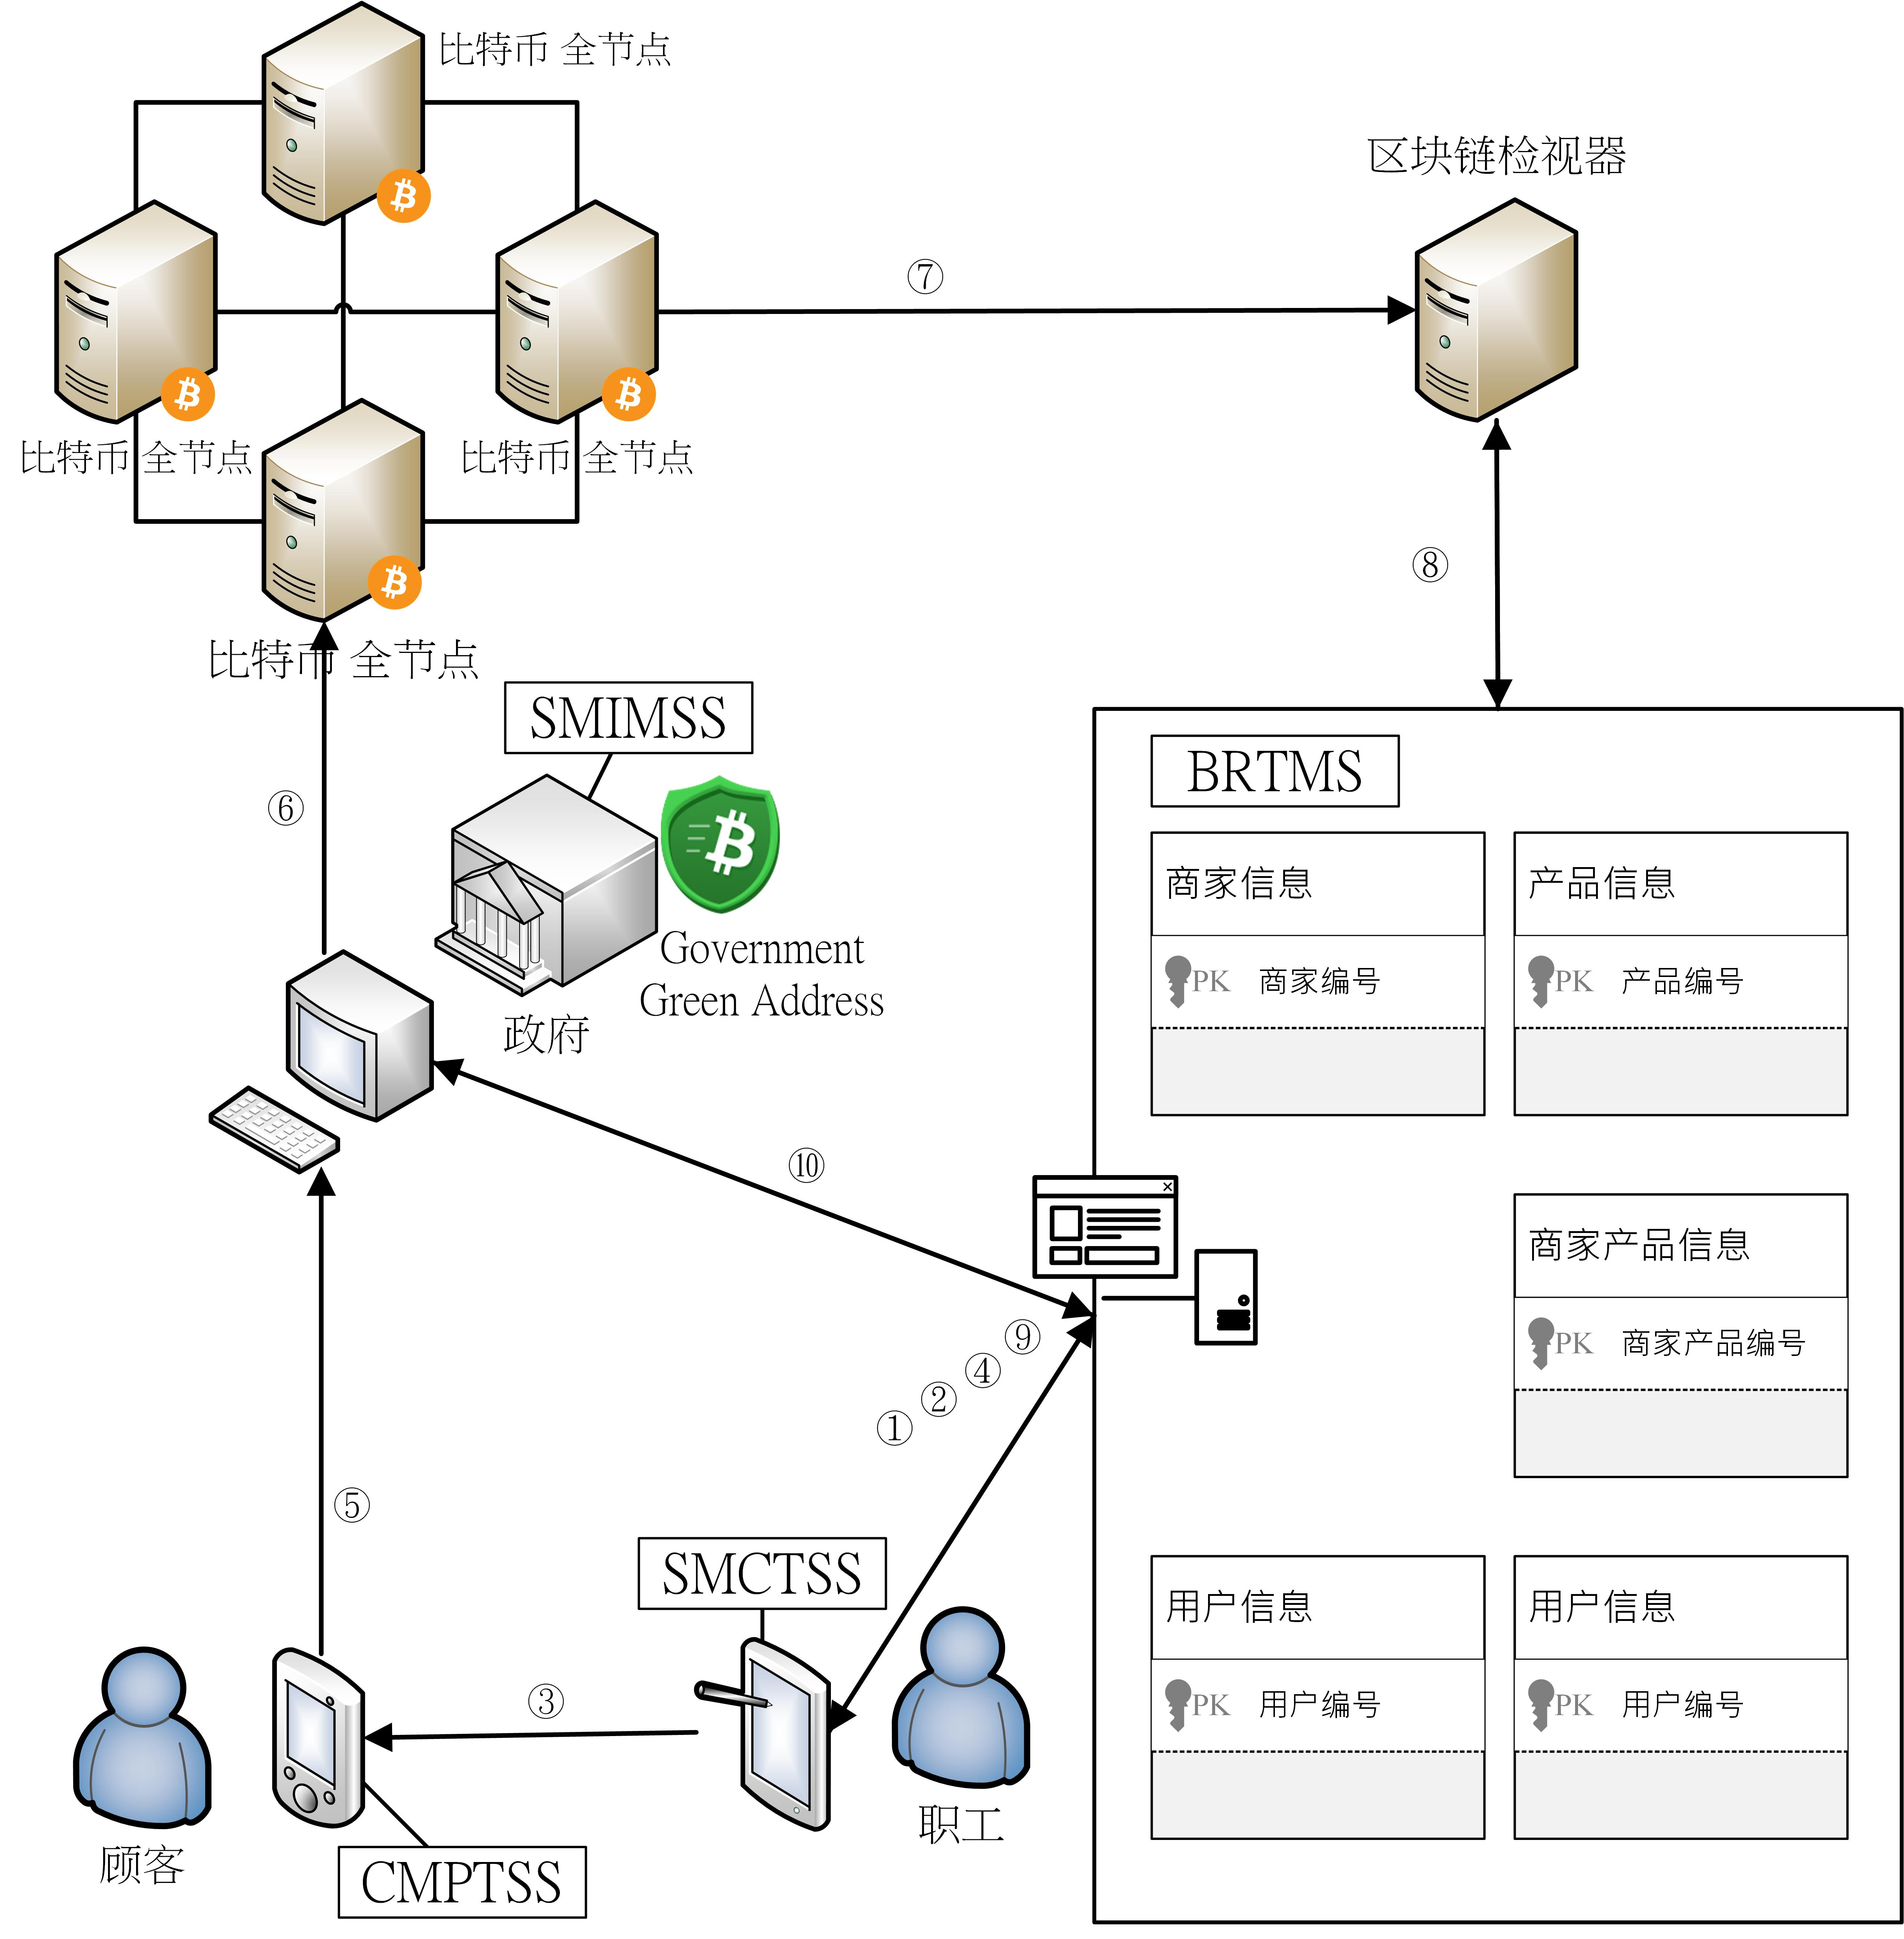
\includegraphics[width = 0.8\textwidth]{gabpcss.jpg}
		\caption{基於Government Green Address的BRTMS整體示意圖}\label{gabpcss}
	\end{figure}

	\begin{enumerate}
		\item 商家以通過政府機構的審查稽覈的用戶登入該系統。
		\item 系統載入該商家註冊的商品信息,職工可以依照顧客的需求進行點單選取數量。
		\item 快速建立交易清單,並透過Government Green Address建立一個全新的比特幣收款地址,再以Android Beam的方式將交易信息輕鬆地傳達給顧客。
		\item 在商家職工的平板電腦收到這筆交易信息之後,會對本監督系統重送一個副本進行存檔。該交易信息包括由監督系統所提出的交易流水號、商家編號等信息。
		\item 顧客收到交易信息後,手機會自動開啟Government Green Address的付款頁面,確認金額無誤之後便能進行支付,此時便會以顧客的比特幣私鑰簽署交易,並等待Government Green Address機構節點的認證及發布。
		\item Government Green Address節點收到交易請求,並完成驗證非雙重支付攻擊後,以代理節點對應地址的私鑰簽署本次交易,並廣播至比特幣節點中。
		\item 區塊鏈檢視器便會開始分析網絡中所有存在緩存池中的交易,以及已經被記錄到區塊鏈中的交易。
		\item 本交易監督系統會向區塊鏈檢視器查找,檢查該筆交易是否已經存在於緩存池當中,若已經確認進入緩存池,則認定該筆交易成立並完成付款。
		\item 在交易確認之後,便向商家職工的平板電腦送出交易已經成交的信息,此時完成交易,於此同時也將該筆交易信息建置於系統數據庫內。
		\item 後續政府可以連入BRTMS系統檢視交易信息。
	\end{enumerate}